%
% GNU courseware, XIN YUAN, 2017
%

\documentclass[11pt]{beamer}
\usepackage{beamerthemesplit}
\usepackage{graphicx}
\usepackage{colortbl}
\usepackage[BoldFont,SlantFont,CJKchecksingle]{xeCJK}
\setCJKmainfont[BoldFont=SimHei,SlantedFont=KaiTi]{SimSun}
\setCJKsansfont[BoldFont=SimHei,SlantedFont=KaiTi]{SimSun}
\setCJKmonofont[ItalicFont={Adobe Fangsong Std}]{SimSun}
\setCJKfamilyfont{zhsong}{SimSun}
%\setCJKfamilyfont{zhhei}{Adobe Song Std}
\setCJKfamilyfont{zhhei}{SimHei}
%\setCJKfamilyfont{zhhei}{Adobe Heiti Std}
\setCJKfamilyfont{zhkai}{KaiTi}
\setCJKfamilyfont{zhfs}{FangSong}
\setCJKfamilyfont{zhls}{LiSu}
\setCJKfamilyfont{zhyy}{YouYuan}
\usetheme{warsaw}

\parindent 2em

%title
\title{生物智能与算法}
\author{袁昕}
\date{\today}

\begin{document}

%title
\frame{\titlepage}

\frame{
\centerline{\textbf{\Huge{课程介绍}}}
}

%tables

\section*{大纲}

\frame{\tableofcontents}

%introduction

\section{简介}
\subsection{定义}

\frame{\frametitle{简介}
计算智能也被称作“软计算”,是根据自然界生物体系的原理和规律,
模仿设计出具有记忆、学习、适应等特性的求解算法的总称。

~

这些算法通过计算机模拟,再现了生物的某些智能行为。
}

%methods

\section{方法}

\frame{\frametitle{方法}
	\begin{itemize}
		\item<1-> 进化(演化)算法(遗传算法,协同进化)
		\item<2-> 免疫算法
		\item<3-> 模拟退火(源自物理)
		\item<4-> 群集智能(蚁群算法,粒子群算法,飞鸟,鱼群,布谷鸟,蝙蝠,萤火虫)
		\item<5-> 人工神经网络(连接型,模糊粗糙,记忆型,脉冲耦合,机器学习,深度)
	\end{itemize}
}

\frame{\frametitle{方法}
	\begin{itemize}
		\item<1-> 专家系统
		\item<2-> 生态动力系统
		\item<3-> 复杂网络和动力学
	\end{itemize}
}

\frame{\frametitle{方法}
都是\textsl{仿生算法}。

~

其最大特点就是不需要建立问题本身精确的数学模型,
适合于解决那些因为难以建立有效的形式化模型而用传统人工智能技术
又难以有效解决甚至无法解决的问题。
}

\frame{\frametitle{优点}

{\CJKfamily{zhfs}
智能计算还具有简单、通用、鲁棒性强、适于并行处理的优点,
使其在并行搜索、联想记忆、模式识别、知识自动获取等方面得到了广泛的应用。
}

~

本课目的之一,要能说出各种方法的\textbf{本质}和\textbf{思维共性}。
}

\frame{\frametitle{缺点}

本课目的之一,要能说出每种方法的假设、缺点和适用范围。
}

\frame{\frametitle{与传统人工智能对比}

{\CJKfamily{zhhei}
计算智能有别于传统的符号智能。符号智能是以知识为基础,通过推理进行问题求解,也即传统的人工智能;
而计算智能则是以数据为基础,通过训练建立联系,进行问题求解。
}

~

{\CJKfamily{zhkai}
计算智能是以联接主义为主的思维方式,即研究简单个体如何在简单交互规则指导下,
构成具有复杂智能行为的高层系统。
}

~

数据驱动,研究相关性为主,因果性为辅。
}

\section{应用}

\frame{\frametitle{应用}

自80年代中后期以来计算智能在众多领域的科学家加入下得到了极大的发展。

~

\textcolor{blue}{看看有哪些应用领域?}
}

\section{工作流程}

\frame{\frametitle{工作流程}
	\begin{enumerate}
		\item<1-> 清晰地描述问题
		\item<2-> 描述数据,识别变量,不变量和隐变量
		\item<3-> 探索量之间的关系,借鉴仿生系统,建立数学模型
		\item<4-> 数字实验和评价
		\item<5-> 对模型进行数学抽象和逻辑分析,给出假设
		\item<6-> 给出直观的几何意义和物理意义
		\item<7-> 和已有方法进行对比,给出优缺点和适用范围
		\item<8-> 撰写报告和论文
	\end{enumerate}
}

\section{课程报告}

\frame{\frametitle{课程报告}
	\begin{enumerate}
		\item 上课时各小组的幻灯或小报告
		\item 每位同学整理一份报告
			\begin{itemize}
				\item 对已有的一个方法的深入阐述,有余力的同学可编程实验并评价
				\item 探索新的方法
				\item 针对科研中的问题,提出计算智能方法并试验
			\end{itemize}
		\item 协作网址或报告发邮件给 `yxxinyuan@zju.edu.cn`
	\end{enumerate}
}

\frame{\frametitle{报告形式}
\begin{minipage}[t]{\textwidth}
幻灯和报告可充分应用图形摘要、漫画等趣味形式,形成既科普,又专业的作品。
\end{minipage}

\uncover<2->{
\begin{minipage}[b]{\textwidth}
\begin{figure}[hb]
\centering
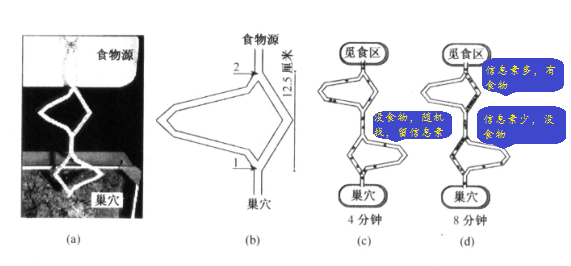
\includegraphics[width=0.8\textwidth]{0-files/ant.png}
\end{figure}
\end{minipage}
}
}

\frame{\frametitle{算法对比}

\begin{table}[htbp]
\centering
\begin{tabular}{|l|c|r|}
\hline
算法   &  精度    &  运算时间(s)\\
\hline
蚁群   &  90\%    &  10.3\\
\hline
\rowcolor[rgb]{0.0, 0.8, 0.8}
进化   &  \textcolor[rgb]{1.0, 1.0, 0.0}{91.2\%}  &  20.6\\
\hline
免疫   &  93.1\%  &  15.9\\
\hline
\end{tabular}
\end{table}
}

\frame{\frametitle{结束}

\centerline{\textbf{\Huge{结束!}}}
}

\frame{\frametitle{版权申明}

本作品采用知识共享 署名-非商业性使用-禁止演绎 3.0 中国大陆 许可协议进行许可。
要查看该许可协议,可访问 http://creativecommons.org/licenses/by-nc-nd/3.0/cn/ 或者
写信到 Creative Commons, PO Box 1866, Mountain View, CA 94042, USA。
}

\end{document}
